% Created 2021-04-20 Tue 19:43
% Intended LaTeX compiler: pdflatex

\documentclass[english]{article}
\usepackage[T1, T2A]{fontenc}
\usepackage[lutf8]{luainputenc}
\usepackage[english, russian]{babel}
\usepackage{minted}
\usepackage{graphicx}
\usepackage{longtable}
\usepackage{hyperref}
\usepackage{xcolor}
\usepackage{natbib}
\usepackage{amssymb}
\usepackage{stmaryrd}
\usepackage{amsmath}
\usepackage{caption}
\usepackage{mathtools}
\usepackage{amsthm}
\usepackage{tikz}
\usepackage{grffile}
\usepackage{extarrows}
\usepackage{wrapfig}
\usepackage{algorithm}
\usepackage{algorithmic}
\usepackage{lipsum}
\usepackage{rotating}
\usepackage{placeins}
\usepackage[normalem]{ulem}
\usepackage{amsmath}
\usepackage{textcomp}
\usepackage{capt-of}


\usepackage{geometry}
\geometry{a4paper,left=2.5cm,top=2cm,right=2.5cm,bottom=2cm,marginparsep=7pt, marginparwidth=.6in}
 \usepackage{hyperref}
 \hypersetup{
     colorlinks=true,
     linkcolor=blue,
     filecolor=orange,
     citecolor=black,
     urlcolor=blue,
     }

\date{}
\title{}
\hypersetup{
 pdfauthor={},
 pdftitle={},
 pdfkeywords={},
 pdfsubject={},
 pdfcreator={Emacs 28.0.50 (Org mode 9.4.4)},
 pdflang={English}}
\begin{document}

\begin{titlepage}
  \begin{center}
    \large\textbf{Федеральное государственное автономное образовательное учреждение высшего образования ``Национальный исследовательский университет ИТМО``} \\
    \vspace{0.5cm}
    Факультет информационных технологий и программирования \\
    \vspace{0.5cm}
    Направление ``Прикладная математика и информатика`` \\
    \vspace{3cm}
    Отчет к лабораторной работе №3 \\
    \vspace{0.5cm}
    \textbf{Методы решения систем линейных уравнений}
  \end{center}
  \vfill
  \begin{flushright}
    \large
    Выполнили студенты группы М3237 \\
    \vspace{0.5cm}
    Ярошевский Илья \\
    Аникина Вероника \\
    Крюков Александр
  \end{flushright}
  \vspace{3cm}
  \begin{center}
    Санкт-Петербург 2021
  \end{center}
\end{titlepage}

\section{Цели работы}

\begin{enumerate}
    \item Реализовать прямой метод решения СЛАУ на основе \(LU\)-разложения
    \item Провести исследование метода на матрицах, число обусловленности которых регулируется за счёт изменения диагонального  преобладания
    \item Провести исследование метода на матрицы Гильберта различной размерности
    \item Реализовать метод Гаусса с выбором ведущего элемента для плотных матриц
\end{enumerate}
\section{Ход работы}
Матрицы с диагональным преобладанием строились так:
\[ a_{ii} = \begin{cases}
  -\sum\limits_{i \neq j} a_{ij} & i > 1 \\
  -\sum\limits_{i \neq j} a_{ij} + 10^{-k} & i = 1
\end{cases} \]
, где \(a_{ij} \in \{0, -1, -2, -3, -4\}: i \neq j \) выбиралось
случайным образом. Также задавалось максимальное расстояние от главной
диагонали, дальше которого все элементы были нулевыми. Это позволяет
использовать меньше памяти, за счёт хранения матрицы, в которой ненулевые
элементы расположены близко к главной диагонали, в профильном
формате.

Матрицы Гильберта строились по формуле: \(a_{ij} = \frac{1}{i + j -
  1}, i,j = \overline{1, n}\). Для таких плотных матриц несущественно,
в какой форме их хранить, так как в любом случае потребуется
\(O(n^2)\) памяти

\subsection{Прямой метод}
\subsubsection{Оценка количества операций}
Оценим количество операций умножения и деления для матрицы размера \(n\)
\begin{itemize}
\item Сложность LU-разложения:
\[ \sum_{i=2}^{n} (\sum_{j=1}^{i - 1} (2 \cdot \sum_{k=1}^{j-1} 1) + \sum_{k=1}^{i-1} 1) =\]
\[ \sum_{i=2}^{n} (\sum_{j=1}^{i - 1} (2 \cdot j) + i) =\]
\[ \sum_{i=2}^{n} ((i - 1) \cdot i + i) =\]
\[ \sum_{i=2}^{n} (i^2) =\]
\[ \frac{n^3}{3} + \frac{n^2}{2} + \frac{n}{6} - 1\]
\item Сложность "прямого"\ хода метода Гаусса (упрощенный алгоритм, работающий только для нижнетреугольных матриц):
\[ \sum_{i=1}^{n} (1 + \sum_{j=i+1}^{n} 2) = n^2\]
\item Сложность обратного хода метода Гаусса:
\[ \sum_{i=1}^{n} (1 + \sum_{j=1}^{i-1} 2) =\]
\[ \sum_{i=1}^{n} (2 \cdot i + 1) =\]
\[ n^2 + 2 \cdot n\]

Если при этом учитывать, что на главной диагонали в матрице U стоят единичные элементы, сложность составит
\[ \sum_{i=1}^{n} (1 + \sum_{j=1}^{i-1} 1) =\]
\[ \sum_{i=1}^{n} (i + 1) =\]
\[ \frac{n^2}{2} + 3 \cdot \frac{n}{2}\]
\end{itemize}
Так как в методе каждый из вышеперечисленных алгоритмов исполняется ровно по одному разу, итоговое количество операций составит:
\[ \frac{n^3}{3} + 2 \cdot n^2 + 5 \cdot \frac{n}{3} - 1\]
\subsubsection{Тестирование на матрицах с диагональным преобладание}
\begin{center}
    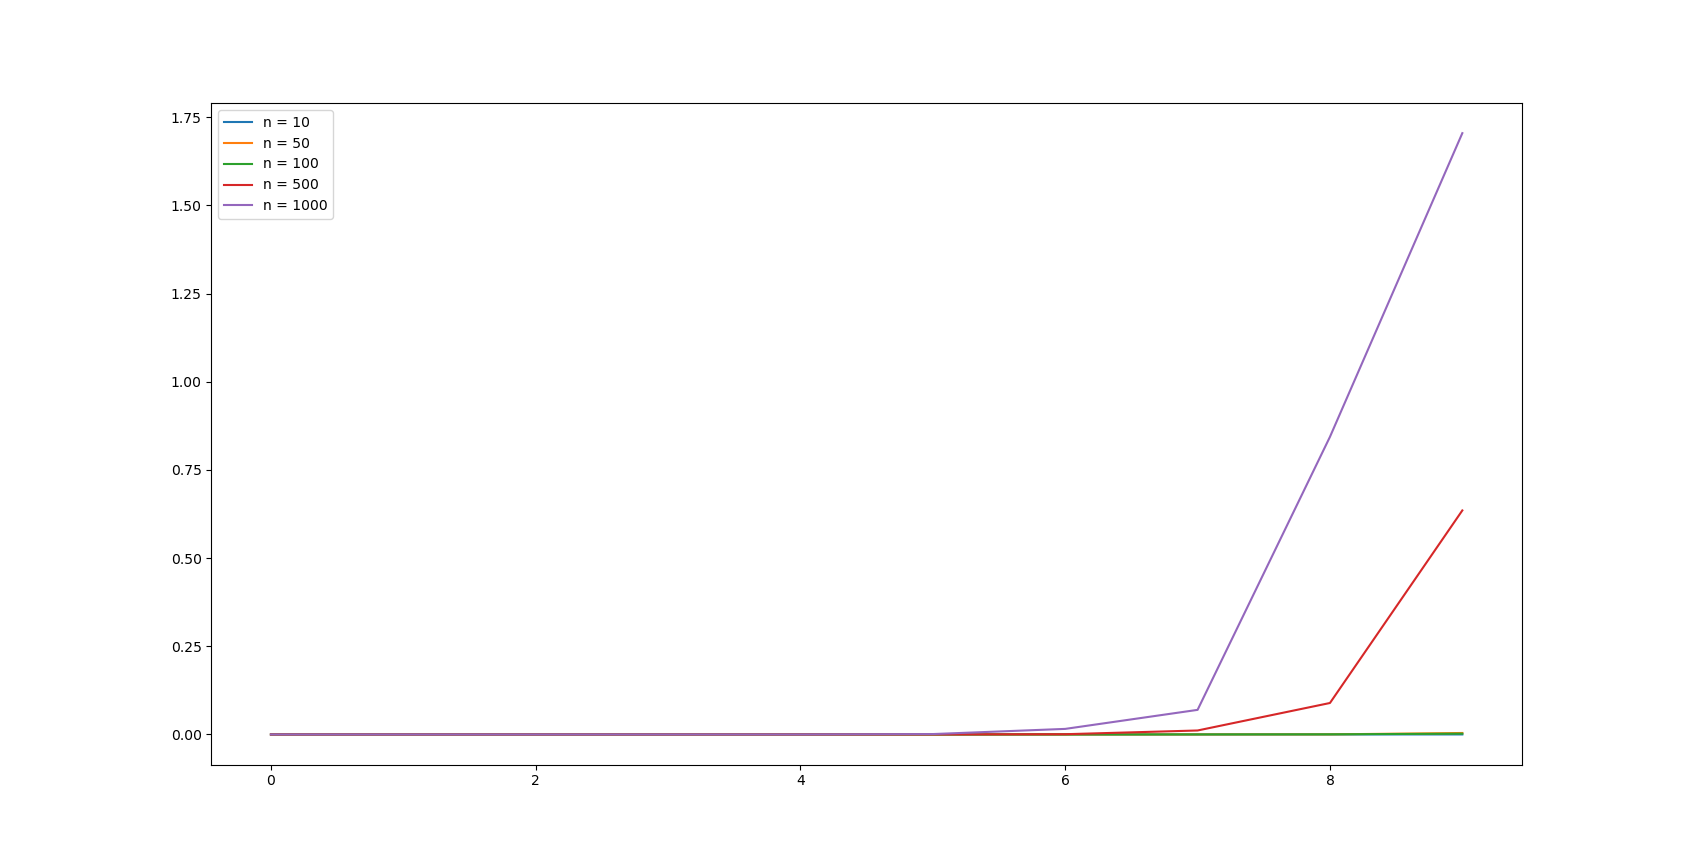
\includegraphics[scale=0.4]{direct.png}
\end{center}
\begin{center}
  \begin{longtable}{l|l|c|c|c}
    \(n\) & \(k\) & \(\Vert x^* - x_k \Vert\) & \(\frac{\Vert x^* - x_k \Vert}{\Vert x^* \Vert}\) & Количество операций\\
    \hline
    10 & 0 & \(5.46103\cdot 10^{-14} \)& \(2.7832\cdot 10^{-15}\) & \\
    10 & 1 & \(1.43296\cdot 10^{-13} \)& \(7.30302\cdot 10^{-15}\) & \\
    10 & 2 & \(3.46274\cdot 10^{-12} \)& \(1.76478\cdot 10^{-13}\) & \\
    10 & 3 & \(1.29306\cdot 10^{-11} \)& \(6.59007\cdot 10^{-13}\) & \\
    10 & 4 & \(3.44677\cdot 10^{-10} \)& \(1.75664\cdot 10^{-11}\) & \({\large 569}\) \\
    10 & 5 & \(1.29248\cdot 10^{-9} \)& \(6.5871\cdot 10^{-11}\) & \\
    10 & 6 & \(3.30301\cdot 10^{-8} \)& \(1.68337\cdot 10^{-9}\) & \\
    10 & 7 & \(5.74436\cdot 10^{-7} \)& \(2.92759\cdot 10^{-8}\) & \\
    10 & 8 & \(8.32931\cdot 10^{-6} \)& \(4.24501\cdot 10^{-7}\) & \\
    10 & 9 & \(1.43609\cdot 10^{-6} \)& \(7.31898\cdot 10^{-8}\) & \\
    \hline
    50 & 0 & \(1.14086\cdot 10^{-12} \)& \(5.50651\cdot 10^{-15}\) & \\
    50 & 1 & \(4.26714\cdot 10^{-13} \)& \(2.0596\cdot 10^{-15}\) & \\
    50 & 2 & \(2.93195\cdot 10^{-10} \)& \(1.41515\cdot 10^{-12}\) & \\
    50 & 3 & \(2.0648\cdot 10^{-9}  \)& \(9.96604\cdot 10^{-12}\) & \\
    50 & 4 & \(6.88083\cdot 10^{-9} \)& \(3.32113\cdot 10^{-11}\) & \({\large 4.6849 \cdot 10^4}\) \\
    50 & 5 & \(1.4312\cdot 10^{-7}  \)& \(6.90788\cdot 10^{-10}\) & \\
    50 & 6 & \(1.83487\cdot 10^{-8} \)& \(8.85625\cdot 10^{-11}\) & \\
    50 & 7 & \(2.38532\cdot 10^{-5} \)& \(1.15131\cdot 10^{-7}\) & \\
    50 & 8 & \(0.000193578 \)& \(9.34332\cdot 10^{-7}\) & \\
    50 & 9 & \(0.00413754  \)& \(1.99704\cdot 10^{-5}\) & \\
    \hline
    100 & 0 & \(9.65618\cdot 10^{-12} \)& \(1.66005\cdot 10^{-14}\) & \\
    100 & 1 & \(1.06903\cdot 10^{-10} \)& \(1.83783\cdot 10^{-13}\) & \\
    100 & 2 & \(6.80943\cdot 10^{-10} \)& \(1.17065\cdot 10^{-12}\) & \\
    100 & 3 & \(9.96402\cdot 10^{-9} \)& \(1.71298\cdot 10^{-11}\) & \\
    100 & 4 & \(4.38007\cdot 10^{-8} \)& \(7.53005\cdot 10^{-11}\) & \({\large 3.53699\cdot 10^6}\) \\
    100 & 5 & \(1.54526\cdot 10^{-6} \)& \(2.65656\cdot 10^{-9}\) & \\
    100 & 6 & \(1.16246\cdot 10^{-6} \)& \(1.99846\cdot 10^{-9}\) & \\
    100 & 7 & \(6.24677\cdot 10^{-5} \)& \(1.07392\cdot 10^{-7}\) & \\
    100 & 8 & \(0.0003323   \)& \(5.71277\cdot 10^{-7}\) & \\
    100 & 9 & \(0.00224864  \)& \(3.86579\cdot 10^{-6}\) & \\
    \hline
    500 & 0 & \(1.59548\cdot 10^{-11} \)& \(2.46801\cdot 10^{-15}\) & \\
    500 & 1 & \(3.26512\cdot 10^{-9} \)& \(5.05073\cdot 10^{-13}\) & \\
    500 & 2 & \(1.2449\cdot 10^{-7}  \)& \(1.9257\cdot 10^{-11}\) & \\
    500 & 3 & \(5.4828\cdot 10^{-8}  \)& \(8.4812\cdot 10^{-12}\) & \\
    500 & 4 & \(1.14655\cdot 10^{-5} \)& \(1.77358\cdot 10^{-9}\) & \({\large 4.2168499 \cdot 10^{7}}\) \\
    500 & 5 & \(6.59951\cdot 10^{-5} \)& \(1.02086\cdot 10^{-8}\) & \\
    500 & 6 & \(0.000661574 \)& \(1.02337\cdot 10^{-7}\) & \\
    500 & 7 & \(0.0112052   \)& \(1.73331\cdot 10^{-6}\) & \\
    500 & 8 & \(0.0891671   \)& \(1.3793\cdot 10^{-5}\) & \\
    500 & 9 & \(0.635155    \)& \(9.82504\cdot 10^{-5}\) & \\
    \hline
    1000 & 0 & \(2.48326\cdot 10^{-8} \)& \(1.35912\cdot 10^{-12}\) & \\
    1000 & 1 & \(1.55912\cdot 10^{-8} \)& \(8.53328\cdot 10^{-13}\) & \\
    1000 & 2 & \(3.0785\cdot 10^{-7}  \)& \(1.6849\cdot 10^{-11}\) & \\
    1000 & 3 & \(1.72248\cdot 10^{-5} \)& \(9.42737\cdot 10^{-10}\) & \\
    1000 & 4 & \(2.15435\cdot 10^{-5} \)& \(1.1791\cdot 10^{-9}\) & \({\large 3.35336999 \cdot 10^8 }\) \\
    1000 & 5 & \(0.00109214  \)& \(5.97744\cdot 10^{-8}\) & \\
    1000 & 6 & \(0.0157364   \)& \(8.6127\cdot 10^{-7}\) & \\
    1000 & 7 & \(0.0697018   \)& \(3.81486\cdot 10^{-6}\) & \\
    1000 & 8 & \(0.843813    \)& \(4.61829\cdot 10^{-5}\) & \\
    1000 & 9 & \(1.70491     \)& \(9.33118\cdot 10^{-5}\)
  \end{longtable}
\end{center}
Можно заметить, что точность значительно уменьшается при увеличении
как размерности пространства, так и числа \(k\). Накопление
погрешности происходит из-за слагаемого \(10^{-k}\), при уменьшении
которого теряется точность вычислений. Стоит заметить, что при больших
размерностях точность теряется быстрее, из-за прибавления \(10^{-k}\)
к большому числу, которое растет с увеличением размерности матрицы.

\subsubsection{Тестирование на матрицах Гильберта}
\begin{center}
  \begin{longtable}{l|l|l}
    \(n\) & \(\Vert x^* - x_k \Vert\) & \(\frac{\Vert x^* - x_k \Vert}{\Vert x^* \Vert}\) \\
    \hline
    10 & \(8.25036\cdot 10^{-9}\) & \(4.20477\cdot 10^{-10}\) \\
    50 & \(7.52844\cdot 10^{-7}\) & \(3.63371\cdot 10^{-9}\) \\
    100 & \(3.95193\cdot 10^{-6}\) & \(6.79401\cdot 10^{-9}\) \\
    500 & \(0.000432803\) & \(6.69491\cdot 10^{-8}\) \\
    1000 & \(0.00435918 \) & \(2.38583\cdot 10^{-7}\)
  \end{longtable}
\end{center}

Тестирование на матрицах Гильберта также показывает уменьшение
точности решения с увеличением размерности, из-за того что деление на
большие числа приводит к уменьшению точности вычисляемого элемента.

\subsection{Метод Гаусса с выбором ведущего элемента}
\subsubsection{Оценка количества операций}
Для матрицы размера \(n\) количество операций при решении уравнения методом Гаусса с выбором ведущего элемента будет равно:
\[ \sum_{i=1}^{n} \sum_{j=i + 1}^{n} (2 + \sum_{k=i+1}^{n} 1) + n^2 + 2\cdot n =\]
\[ \sum_{i=1}^{n} \sum_{j=i + 1}^{n} (2 + n - i) + n^2 + 2\cdot n =\]
\[ \sum_{i=1}^{n} (n - i)\cdot (2 + n - i) + n^2 + 2\cdot n =\]
\[ \frac{n \cdot (2 \cdot n^2 + \frac{n^2}{2} + 7 \cdot \frac{n}{6})}{6} + n^2 + 2 \cdot n =\]
\[ \frac{n^3}{3} + 3 \cdot \frac{n^2}{2} + 7 \cdot \frac{n}{6}\]
\subsubsection{Тестирование на матрицах с диагональным преобладание}
\begin{center}
    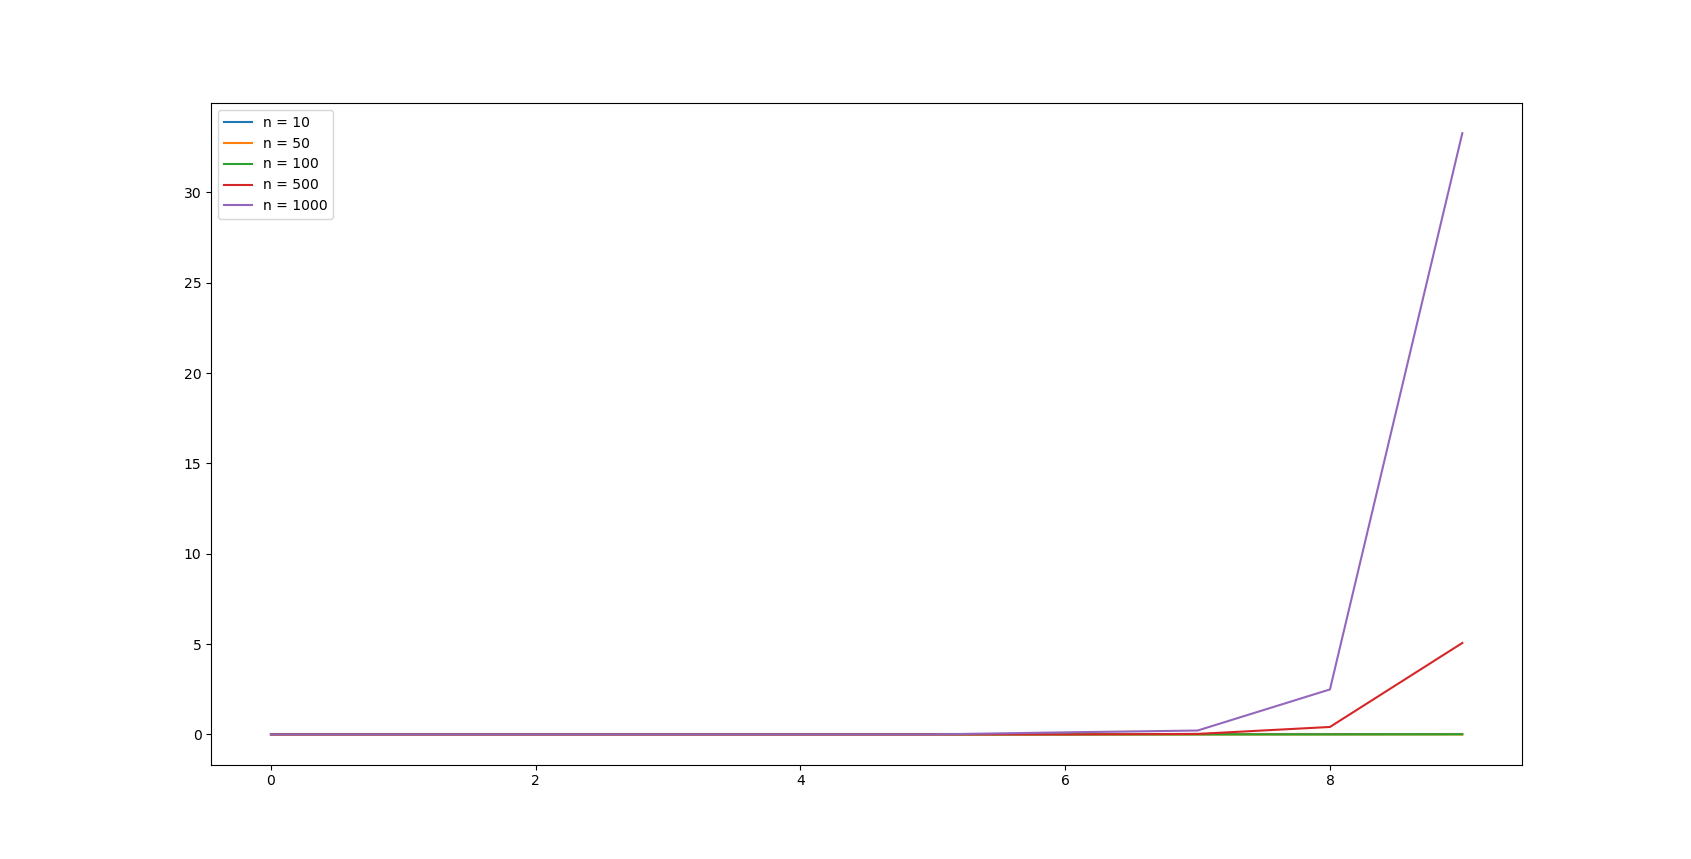
\includegraphics[scale=0.4]{main_elem.png}
\end{center}
\begin{center}
  \begin{longtable}{l|l|c|c|c}
    \(n\) & \(k\) & \(\Vert x^* - x_k \Vert\) & \(\frac{\Vert x^* - x_k \Vert}{\Vert x^* \Vert}\) & Количество операций\\
    \hline
    10 & 0 & \(6.32562\cdot 10^{-14}\) & \(3.22384\cdot 10^{-15}\) & \\
    10 & 1 & \(1.60765\cdot 10^{-13}\) & \(8.19336\cdot 10^{-15}\) & \\
    10 & 2 & \(2.30718\cdot 10^{-12}\) & \(1.17585\cdot 10^{-13}\) & \\
    10 & 3 & \(1.2928\cdot 10^{-11}\) & \(6.58874\cdot 10^{-13}\) & \\
    10 & 4 & \(7.32431\cdot 10^{-10}\) & \(3.73281\cdot 10^{-11}\) & \({\large 240}\)\\
    10 & 5 & \(4.16467\cdot 10^{-9}\) & \(2.12251\cdot 10^{-10}\) & \\
    10 & 6 & \(7.18045\cdot 10^{-9}\) & \(3.6595\cdot 10^{-10}\) & \\
    10 & 7 & \(1.43609\cdot 10^{-7}\) & \(7.31899\cdot 10^{-9}\) & \\
    10 & 8 & \(5.45714\cdot 10^{-6}\) & \(2.78121\cdot 10^{-7}\) & \\
    10 & 9 & \(1.00526\cdot 10^{-5}\) & \(5.12329\cdot 10^{-7}\) & \\
    \hline
    50 & 0 & \(3.39627\cdot 10^{-12}\) & \(1.63926\cdot 10^{-14}\) & \\
    50 & 1 & \(7.07182\cdot 10^{-11}\) & \(3.41331\cdot 10^{-13}\) & \\
    50 & 2 & \(6.73371\cdot 10^{-10}\) & \(3.25012\cdot 10^{-12}\) & \\
    50 & 3 & \(1.86195\cdot 10^{-8}\) & \(8.98695\cdot 10^{-11}\) & \\
    50 & 4 & \(5.47724\cdot 10^{-8}\) & \(2.64366\cdot 10^{-10}\) & \({\large 3.92 \cdot 10^4}\) \\
    50 & 5 & \(9.17442\cdot 10^{-9}\) & \(4.42816\cdot 10^{-11}\) & \\
    50 & 6 & \(4.27524\cdot 10^{-6}\) & \(2.0635\cdot 10^{-8}\) & \\
    50 & 7 & \(3.20184\cdot 10^{-5}\) & \(1.54541\cdot 10^{-7}\) & \\
    50 & 8 & \(0.0010422\) & \(5.03031\cdot 10^{-6}\) & \\
    50 & 9 & \(0.00196329\) & \(9.4761\cdot 10^{-6}\) & \\
    \hline
    100 & 0 & \(9.19552\cdot 10^{-12}\) & \(1.58086\cdot 10^{-14}\) & \\
    100 & 1 & \(1.67913\cdot 10^{-10}\) & \(2.8867\cdot 10^{-13}\) & \\
    100 & 2 & \(5.97625\cdot 10^{-11}\) & \(1.02741\cdot 10^{-13}\) & \\
    100 & 3 & \(3.8314\cdot 10^{-9}\) & \(6.5868\cdot 10^{-12}\) & \\
    100 & 4 & \(5.50153\cdot 10^{-8}\) & \(9.45803\cdot 10^{-11}\) & \(\large 3.234 \cdot 10^5\) \\
    100 & 5 & \(2.62084\cdot 10^{-6}\) & \(4.50565\cdot 10^{-9}\) & \\
    100 & 6 & \(9.08835\cdot 10^{-6}\) & \(1.56243\cdot 10^{-8}\) & \\
    100 & 7 & \(0.000175778\) & \(3.02191\cdot 10^{-7}\) & \\
    100 & 8 & \(0.000469095\) & \(8.06451\cdot 10^{-7}\) & \\
    100 & 9 & \(0.00579465\) & \(9.96195\cdot 10^{-6}\) & \\
    \hline
    500 & 0 & \(4.74104\cdot 10^{-9}\) & \(7.33379\cdot 10^{-13}\) & \\
    500 & 1 & \(5.09336\cdot 10^{-8}\) & \(7.87879\cdot 10^{-12}\) & \\
    500 & 2 & \(2.70421\cdot 10^{-7}\) & \(4.18307\cdot 10^{-11}\) & \\
    500 & 3 & \(4.62975\cdot 10^{-6}\) & \(7.16164\cdot 10^{-10}\) & \\
    500 & 4 & \(3.53666\cdot 10^{-5}\) & \(5.47076\cdot 10^{-9}\) & \(\large 4.1417 \cdot 10^7 \) \\
    500 & 5 & \(0.000144481\) & \(2.23495\cdot 10^{-8}\) & \\
    500 & 6 & \(0.000741575\) & \(1.14712\cdot 10^{-7}\) & \\
    500 & 7 & \(0.0285386\) & \(4.41456\cdot 10^{-6}\) & \\
    500 & 8 & \(0.414411\) & \(6.41041\cdot 10^{-5}\) & \\
    500 & 9 & \(5.06399\) & \(0.000783335\) & \\
    \hline
    1000 & 0 & \(5.03021\cdot 10^{-8}\) & \(2.75309\cdot 10^{-12}\) & \\
    1000 & 1 & \(2.34771\cdot 10^{-8}\) & \(1.28493\cdot 10^{-12}\) & \\
    1000 & 2 & \(1.75109\cdot 10^{-6}\) & \(9.58395\cdot 10^{-11}\) & \\
    1000 & 3 & \(4.60324\cdot 10^{-5}\) & \(2.51941\cdot 10^{-9}\) & \\
    1000 & 4 & \(0.000152474\) & \(8.34511\cdot 10^{-9}\) & \(\large 3.32334 \cdot 10^8 \) \\
    1000 & 5 & \(0.000391032\) & \(2.14016\cdot 10^{-8}\) & \\
    1000 & 6 & \(0.116013\) & \(6.34951\cdot 10^{-6}\) & \\
    1000 & 7 & \(0.216661\) & \(1.18581\cdot 10^{-5}\) & \\
    1000 & 8 & \(2.49188\) & \(0.000136384\) & \\
    1000 & 9 & \(33.2835\) & \(0.00182164\)
  \end{longtable}
\end{center}

Здесь также можно наблюдать потерю точности при увеличении размерности
и числа \(k\). Метод Гаусса работает с плотными матрицами, и требует
большего числа операций, что приводит к меньшей точности результата по
сравнению с прямым методом. Для больших размерностей результирующая
погрешность получается достаточно существенной.

\subsubsection{Тестирование на матрицах Гильберта}
\begin{center}
  \begin{longtable}{l|l|l}
    \(n\) & \(\Vert x^* - x_k \Vert\) & \(\frac{\Vert x^* - x_k \Vert}{\Vert x^* \Vert}\) \\
    \hline
    10 & \(4.53743\cdot 10^{-8}\) & \(2.31249\cdot 10^{-9}\) \\
    50 & \(6.4107\cdot 10^{-7} \) & \(3.09422\cdot 10^{-9}\) \\
    100 & \(2.98603\cdot 10^{-6}\) & \(5.13347\cdot 10^{-9}\) \\
    500 & \(0.000384986\) & \(5.95524\cdot 10^{-8}\) \\
    1000 & \(0.00281381 \) & \(1.54003\cdot 10^{-7}\)
  \end{longtable}
\end{center}

На плотных матрицах Гильберта метод Гаусса с выбором главного элемента
показывает меньшую погрешность, чем прямой метод. Точность
увеличивается в \(\approx 2\) раза.

\subsection{Метод сопряженных градиентов}
Для тестирования метода сопряженных градиентов применялся следующий
метод генерирования матриц с диагональным преобладанием:
\[ a_{ii} = \begin{cases}
  \sum\limits_{i \neq j} a_{ij} & i > 1 \\
  \sum\limits_{i \neq j} a_{ij} + 1 & i = 1
\end{cases} \]
, где \(a_{ij}\) и расстояние от главной диагонали выбирались так же,
как и для методов Гаусса. Аналогичным образом генерировались матрицы с
обратным знаком внедиагональных элементов для тестирования метода
Сопряженных градиентов.
\subsubsection{Тестирование на матрицах с диагональным преобладание}

\begin{center}
  \begin{longtable}{l|l|c|c|c}
    \(n\) & Количество итераций & \(\Vert x^* - x \Vert\) & \(\frac{\Vert x^* - x \Vert}{\Vert x^* \Vert}\) & \(\mathop{\rm cond}(A) \)\\
    \hline
    10 & 10 & \(6.52282\cdot 10^{-13}\) & \(3.32434\cdot 10^{-14}\) & \(0.0638468\) \\
    50 & 41 & \(8.95982\cdot 10^{-7}\) & \(4.32458\cdot 10^{-9}\) & \(0.142443\) \\
    100 & 44 & \(6.25949\cdot 10^{-6}\) & \(1.07611\cdot 10^{-8}\) & \(0.153971\) \\
    500 & 85 & \(2.94728\cdot 10^{-5}\) & \(4.55907\cdot 10^{-9}\) & \(0.0545894\) \\
    1000 & 82 & \(7.59348\cdot 10^{-5}\) & \(4.156\cdot 10^{-9}\) & \(0.0502845\) \\
    10000 & 238 & \(0.000528598\) & \(9.15489\cdot 10^{-10}\) & \(0.0134006\) \\
    100000 & 909 & \(0.00839306\) & \(4.59704\cdot 10^{-10}\) & \(0.00494516\)
  \end{longtable}
\end{center}
Погрешность данного метода решения СЛАУ, так же, как в предыдущих методах,
увеличивается с ростом размерности, причем точность
решения сопоставима с точностью у предыдущих методов. Главное преимущество данного метода в том, что он
выполняет
\subsubsection{Тестирование на матрицах с диагональным преобладание с обратным знаком недиагональных элементов}
\begin{center}
  \begin{longtable}{l|l|c|c|c}
    \(n\) & Количество итераций & \(\Vert x^* - x \Vert\) & \(\frac{\Vert x^* - x \Vert}{\Vert x^* \Vert}\) & \(\mathop{\rm cond}(A) \)\\
    \hline
    10 & 10 & \(5.11907\cdot 10^{-12}\) & \(2.60892\cdot 10^{-13}\) & \(0.866552\) \\
    50 & 28 & \(7.79714\cdot 10^{-5}\) & \(3.7634\cdot 10^{-7}\) & \(4.77355\) \\
    100 & 29 & \(0.000204195\) & \(3.51045\cdot 10^{-7}\) & \(3.81639\) \\
    500 & 28 & \(0.00174227\) & \(2.69507\cdot 10^{-7}\) & \(4.77378\) \\
    1000 & 32 & \(0.0122171\) & \(6.68658\cdot 10^{-7}\) & \(7.86291\) \\
    10000 & 38 & \(0.235374\) & \(4.07649\cdot 10^{-7}\) & \(6.09502\) \\
    100000 & 47 & \(7.31364\) & \(4.00582\cdot 10^{-7}\) & \(5.48494\)
  \end{longtable}
\end{center}
Для матриц с неотрицательными внедиагональными элементами можно наблюдать большую погрешность, но в целом меньшее количество итераций.
\subsubsection{Тестирование на матрицах Гильберта}
\begin{center}
  \begin{longtable}{l|l|c|c|c}
    \(n\) & Количество итераций & \(\Vert x^* - x \Vert\) & \(\frac{\Vert x^* - x \Vert}{\Vert x^* \Vert}\) & \(\mathop{\rm cond}(A) \)\\
    \hline
    10 & 5 & 0.311773 & \(0.0158894\) & \(165700\) \\
    50 & 11 & 1.48018 & \(0.00714428\) & \(1.02527 \cdot 10^{6}\) \\
    100 & 14 & 4.02852 & \(0.00692568\) & \(804373\) \\
    500 & 18 & 53.2963 & \(0.00824426\) & \(440191\) \\
    1000 & 21 & 144.311 & \(0.0078983\) & \(421074\)
  \end{longtable}
\end{center}
На плотных матрицах метод сопряженных градиентов даёт очень
большую погрешность, причем она довольно быстро растет с увеличением
размерности матрицы. Стоит отметить, что даже на больших размерностях
метод показывает достаточно малое число итераций как
\section{Выводы}
Самую высокую точность решения на матрицах с диагональным
преобладанием показывает прямой метод Гаусса на основе LU-разложения,
немного менее точен метод Гаусса с выбором главного элемента. Метод
сопряженных градиентов выдает абсолютную погрешность на три порядка
хуже, чем два других метода. На произвольных плотных матрицах метод
Гаусса с выбором главного элемента работает с меньшей погрешностью.

По требуемому количеству памяти на разреженных матрицах лучше всего
показывает себя прямой метод, так как ему достаточно матрицы в
профильной форме. На разреженных симметричных матрицах метод
сопряженных градиентов так же требует малое количество памяти.

По количеству действий метод сопряженных градиентов на больших
размерностях показывает лучшие результаты. Построение матрицы в
разреженном формате выполняется за \(O(n^2)\), на каждой итерации
выполняется два матрично векторных произведений за (\(O(n^2)\)). Заметим,
что количество часто много меньше размерности матрицы, тогда как
другие методы имеют асимптотику \(O(n^3)\).
\end{document}
